\documentclass[a4paper, fleqn]{article}

\usepackage{amsmath}
\usepackage{enumitem}
\usepackage{graphicx}

\begin{document}

\title{Homework I \\ Introduction to Physical Chemistry}
\author{Basil R. Yap 1001690}
\date{2018 January 25}
\maketitle

\section{Question 1}

$\Phi_3 = \left(\frac{2}{L}\right)^{\frac{1}{2}}\sin\left(\frac{3\pi x}{L}\right)$\\
$\begin{aligned}\Pr(0.15L\leq0x\leq0.17L)&=\int_{0.15L}^{0.17L}\left|\Phi_3(x)\right|^2dx\\&=\int_{0.15L}^{0.17L}\left(\frac{2}{L}\right)^{\frac{1}{2}}\sin\left(\frac{3\pi x}{L}\right)\cdot\left(\frac{2}{L}\right)^{\frac{1}{2}}\sin\left(\frac{3\pi x}{L}\right)dx\\&=\frac{2}{L}\int_{0.15L}^{0.17L}\sin^2\left(\frac{3\pi x}{L}\right)dx\end{aligned}$\\
\\
Let $u=\frac{3\pi x}{L},\ du=\frac{3\pi}{L}dx,\ dx=\frac{L}{3\pi}du$\\
\\
$\begin{aligned}\Pr(0.15L\leq0x\leq0.17L)&=\frac{2}{L}\int_{0.45\pi}^{0.51\pi}\frac{L}{3\pi}\sin^2(u)du\\&=\frac{2}{3\pi}\int_{0.45\pi}^{0.51\pi}\frac{1}{2}(1-\cos(2u))du\\&=\frac{1}{3\pi}\left[u-\frac{1}{2}\sin(2u)\right]_{0.45\pi}^{0.51\pi}\\&=0.1733-0.1336\\&=0.0397\end{aligned}$\\

\pagebreak

\section{Question 2}

\begin{enumerate}[label=(\alph{*})]
\item 
$\begin{aligned}\text{ total nodes }&=5\\\text{ total radial nodes }&=5\\\text{ total nodes }&=n-1\\n&=5\\\text{ total radial nodes }&=n-l-1\\l&=0\end{aligned}$\\
The associated orbital is 6s
\item 
$\begin{aligned}\text{ total nodes }&=3\\\text{ total radial nodes }&=0\\\text{ total nodes }&=n-1\\n&=4\\\text{ total radial nodes }&=n-l-1\\l&=3\end{aligned}$\\
The associated orbital is 4f
\end{enumerate}

\pagebreak

\section{Question 3}

\begin{enumerate}[label=(\alph{*})]
\item radial component: $[1-\frac{1}{4}\left(\frac{r}{a_0}\right)+\frac{1}{80}\left(\frac{r}{a_0}\right)^2]\left(\frac{r}{a_0}\right)$\\
$[1-\frac{1}{4}\left(\frac{r}{a_0}\right)+\frac{1}{80}\left(\frac{r}{a_0}\right)^2]\left(\frac{r}{a_0}\right)=0$ where $r\neq0$\\
$\begin{aligned}1-\frac{1}{4}\left(\frac{r}{a_0}\right)+\frac{1}{80}\left(\frac{r}{a_0}\right)^2&=0\\r^2-20a_0r+80a_0^2&=0\\\left(r-10a_0\right)^2-100a_0^2+80a_0^2&=0\\(r-10a_0)^2&=20a_0^2\\r&=10a_0\pm\sqrt{20}a_0\end{aligned}$\\
Radial nodes exist when $r=(10+\sqrt{20})a_0\text{  or  }(10-\sqrt{20})a_0$ .
\item There are two radial nodes
\item angular component: $\sin\theta\sin\phi$\\
$\begin{aligned}\sin\theta\sin\phi&=0\\\end{aligned}$
\item $4p_y$
\item \begin{figure}[h!]
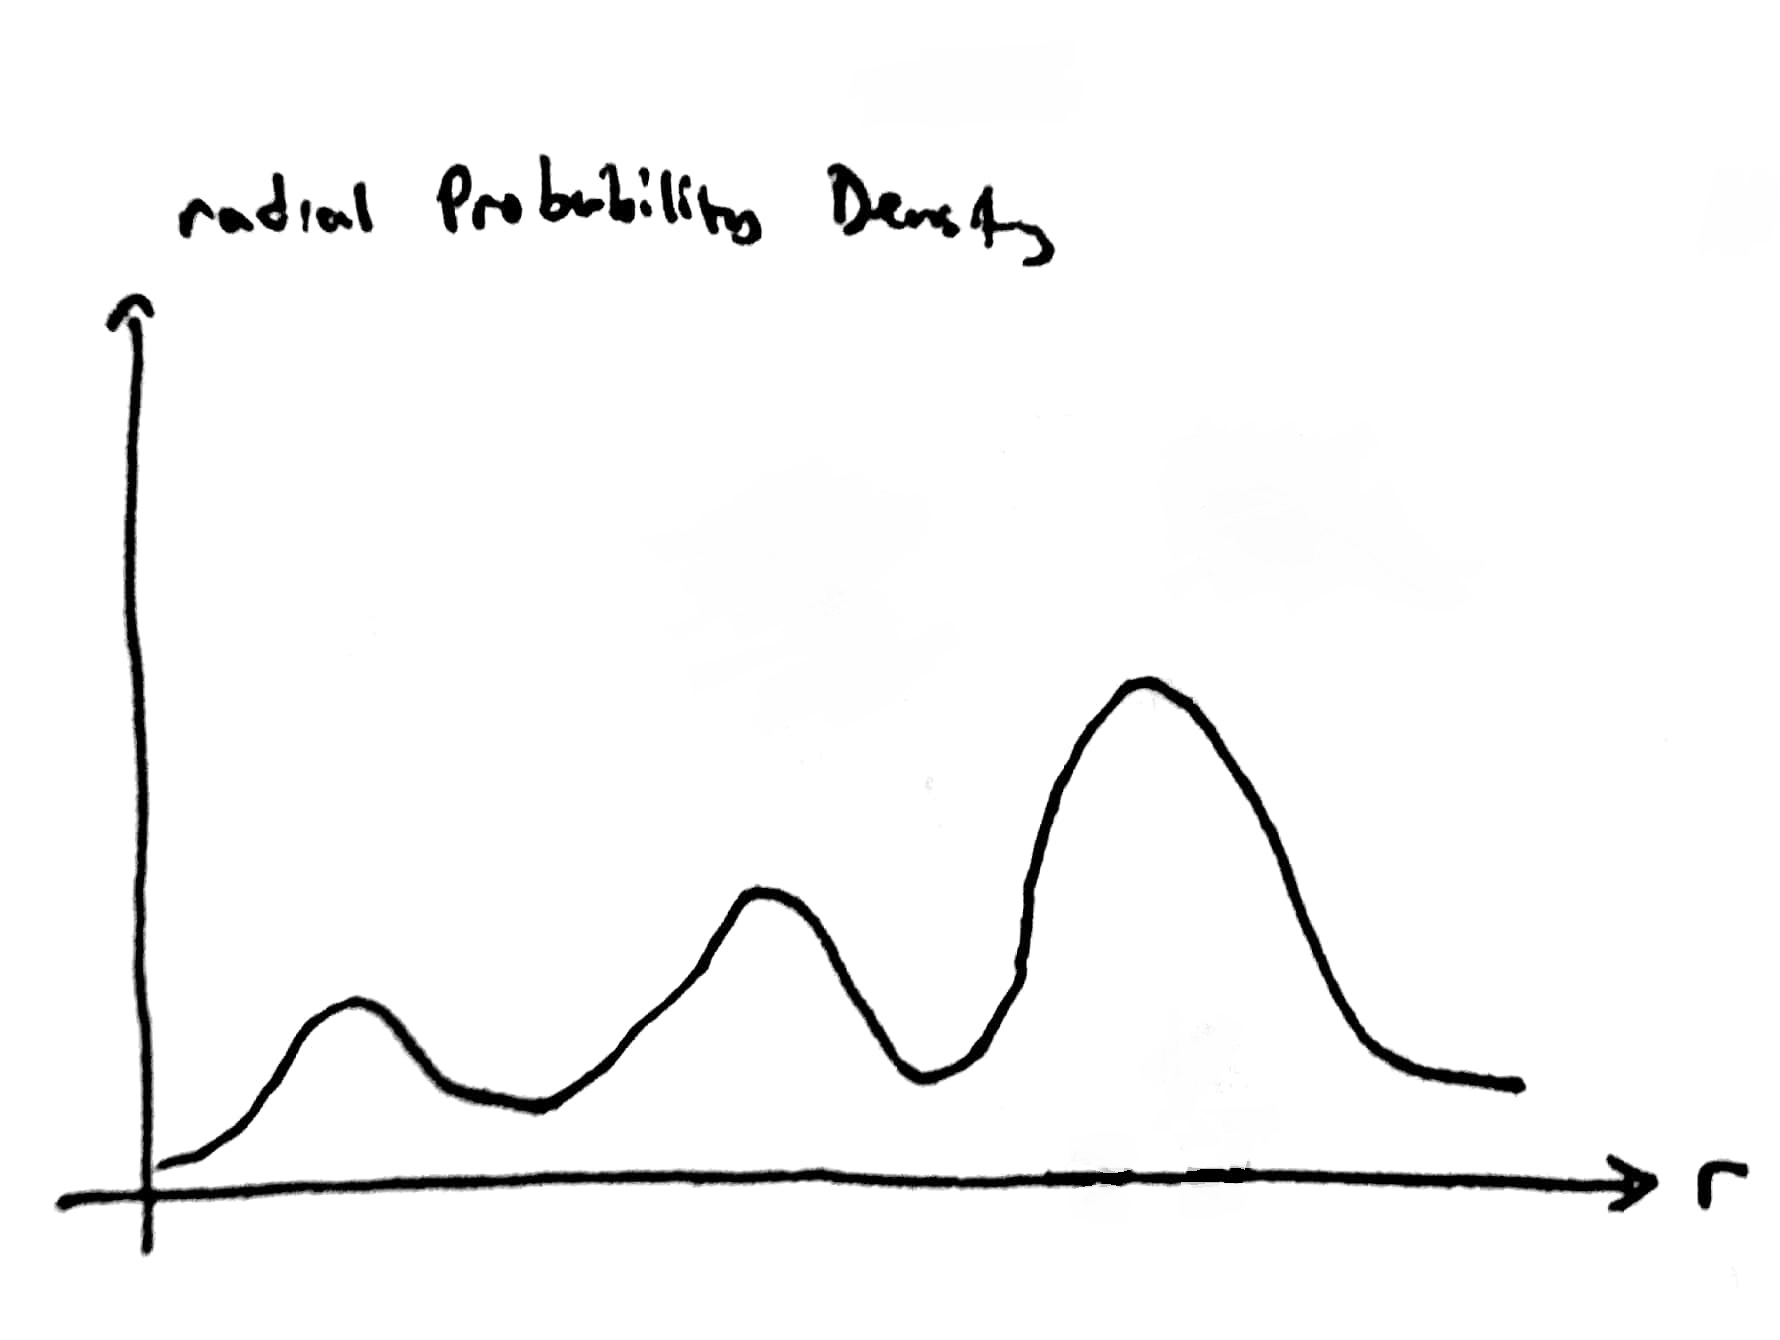
\includegraphics[width=\linewidth]{./assets/201802062208.jpg}
\caption{RPD Graph}
\label{fig:graph3.1}
\end{figure}
\end{enumerate}

\end{document}